\documentclass[../../../main.tex]{subfiles}
\begin{document}

%%%%%%%%%%%%%%%%%%%%%%%%%%%%%%%%%%%%%%%%%
%%%%%%%%%%%%%%%%%%%%%%%%%%%%%%%%%%%%%%%%%
%%%%%%%%%%%%%%%%%%%%%%%%%%%%%%%%%%%%%%%%%
\chapter{Visualizing frequencies}


%%%%%%%%%%%%%%%%%%%%%%%%%%%%%%%%%%%%%%%%%
%%%%%%%%%%%%%%%%%%%%%%%%%%%%%%%%%%%%%%%%%
\section{The shape of the data}

What are frequencies useful for? Statisticians sometimes say that frequencies help us see the \vocab{shape} of the data. They also say frequencies help us see the \vocab{distribution} of the data. These terms ``shape'' and ``distribution'' --- as they are used here --- are synonyms. What this means is that frequencies help us see which values the data clumps around. Or, to put it another way, we can see where the data gets distributed. If we draw a map of the data, so to speak, we can see where the values are distributed on that map. 

Take the Audi R8 colors as an example. In Table \ref{table:R8 colors}, we can see that lots of values are clumped around (or distributed under) the ``white'' color, somewhat less clump around (or are distributed under) the ``black'' color, and so on.

\begin{table}[ht]
  \begin{tabular}{| c | c | c |}
    \hline
    \textbf{Color} & \textbf{Frequency} & \textbf{Relative frequency} \\
    \hline
    Black & 12 & 0.3 (30\%) \\
    \hline
    White & 16 & 0.4 (40\%) \\
    \hline
    Red & 4 & 0.1 (10\%) \\
    \hline
    Yellow & 8 & 0.2 (20\%) \\
    \hline
    Brown & 0 & 0.0 (0\%) \\
    \hline
    \textbf{Total} & 40 & 100\% \\
    \hline
  \end{tabular}
  \caption{\label{table:R8 colors} Colors of Audi R8s sold last year}
\end{table}

There are a number of charts and graphs that help to visualize the shape or distribution of a data set, so that it is easy to see (just by looking) where the values get distributed.


%%%%%%%%%%%%%%%%%%%%%%%%%%%%%%%%%%%%%%%%%
%%%%%%%%%%%%%%%%%%%%%%%%%%%%%%%%%%%%%%%%%
\section{Stem and leaf}

The stem-and-leaf plot is a simple way to begin to see the shape of the frequency counts in a data set. 


%%%%%%%%%%%%%%%%%%%%%%%%%%%%%%%%%%%%%%%%%
\subsection{Digits}

Recall that numbers are typically written with a digit in the ones column, a digit in the tens column, a digit in the hundreds column, and so on. For example, consider the number 123 (one hundred and twenty three). The digit ``3'' sits in the ones column, ``2'' sits in the tens column, and ``1'' sits in the hundreds column. Like this:

\begin{center}
  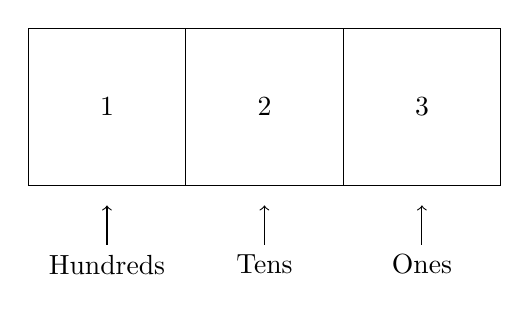
\begin{tikzpicture}

    \draw (0,0) -- (6, 0);
    \draw (6, 0) -- (6, -2);
    \draw (6, -2) -- (0, -2);
    \draw (0, -2) -- (0, 0);
    \draw (2, 0) -- (2, -2);
    \draw (4, 0) -- (4, -2);
    
    \node at (1, -1) {1};
    \node at (3, -1) {2};
    \node at (5, -1) {3};

    \draw[<-] (1, -2.25) -- (1, -2.75);
    \node at (1, -3) {Hundreds};
    \draw[<-] (3, -2.25) -- (3, -2.75);
    \node at (3, -3) {Tens};
    \draw[<-] (5, -2.25) -- (5, -2.75);
    \node at (5, -3) {Ones};

  \end{tikzpicture}
\end{center}

We can add zeros to the left without changing this number. For instance, we could add a zero to the thousands column, to get ``0123,'' like this:

\begin{center}
  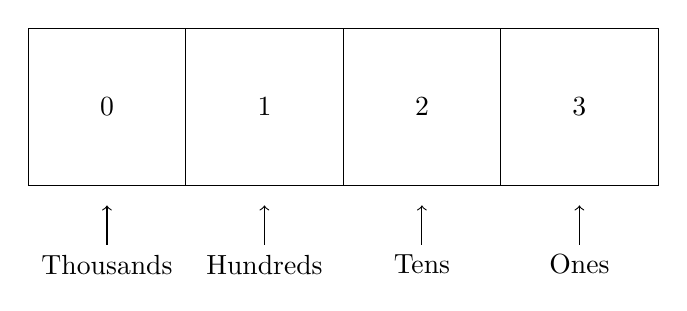
\begin{tikzpicture}

    \draw (0,0) -- (-2, 0);
    \draw (-2,0) -- (-2, -2);
    \draw (-2, -2) -- (0, -2);
    \draw (0,0) -- (6, 0);
    \draw (6, 0) -- (6, -2);
    \draw (6, -2) -- (0, -2);
    \draw (0, -2) -- (0, 0);
    \draw (2, 0) -- (2, -2);
    \draw (4, 0) -- (4, -2);
    
    \node at (-1, -1) {0};
    \node at (1, -1) {1};
    \node at (3, -1) {2};
    \node at (5, -1) {3};

    \draw[<-] (-1, -2.25) -- (-1, -2.75);
    \node at (-1, -3) {Thousands};
    \draw[<-] (1, -2.25) -- (1, -2.75);
    \node at (1, -3) {Hundreds};
    \draw[<-] (3, -2.25) -- (3, -2.75);
    \node at (3, -3) {Tens};
    \draw[<-] (5, -2.25) -- (5, -2.75);
    \node at (5, -3) {Ones};

  \end{tikzpicture}
\end{center}

The zeros on the left don't change the number: ``123'' is the same as ``0123.'' Of course, usually we don't write any extra zeros on the left, but this is just a social convention.


%%%%%%%%%%%%%%%%%%%%%%%%%%%%%%%%%%%%%%%%%
\subsection{Constructing a stem-and-leaf table}

Consider Table \ref{table:R8 colors}. To build a stem-and-leaf plot from that data, first take the frequency counts:

\begin{center}
  12, 16, 4, 8, 0
\end{center}

Next, add zeros on the left wherever needed so that all the numbers have the same number of digits. Like this:

\begin{center}
  12, 16, 04, 08, 00
\end{center}

Now stack these numbers on top of each other, so that they line up vertically. Like this:

\begin{center}
  12 \\
  16 \\
  04 \\
  08 \\
  00
\end{center}

Now split off the ones column. To show what I mean, let's draw a line to separate the ones column from the rest of the digits on the left. For example, with the first number (with is ``16''), draw a line between the ``6'' in the ones column and everything to the left of it, like this: 1~$|$~6. That shows that the digit in the ones column (which is ``6'') is separated off from the numbers on the left (in this case, the ``1'' in the tens column). If we do this for all the numbers, we get this:

\begin{center}
  1~$|$~2 \\
  1~$|$~6 \\
  0~$|$~4 \\
  0~$|$~8 \\
  0~$|$~0
\end{center}

It is easy to see that we have a table:

\begin{center}
  \begin{tabular}{| r | l |}
    \hline
    1 & 2 \\ \hline
    1 & 6 \\ \hline
    0 & 4 \\ \hline
    0 & 8 \\ \hline
    0 & 0 \\ \hline    
  \end{tabular}
\end{center}

Notice that in the left column, there are duplicates. We can consolidate the rows that have the same numbers in the left column by collapsing them into a single row. The way we do this is we put all the digits from the ones column next to each other, in the right column. 

For example, we have two rows that have a ``1'' in the left column. We can collapse these into one row, by putting the digits in the ones column next to each other. So we put the ``2'' and the ``6'' in the right column. Like this:

\begin{center}
  \begin{tabular}{| r | l |}
    \hline
    1 & 2~6 \\ \hline
    0 & 4 \\ \hline
    0 & 8 \\ \hline
    0 & 0 \\ \hline    
  \end{tabular}
\end{center}

Now we can see in the first row that there are \emph{two} values with ``1'' in the tens column. There is ``1'' and ``2'' (i.e., ``12''), and there is ``1'' and ``6'' (i.e., ``16'').

We can collapse the rows that have ``0'' in the tens column too:

\begin{center}
  \begin{tabular}{| r | l |}
    \hline
    1 & 2~6 \\ \hline
    0 & 0~4~8 \\ \hline
  \end{tabular}
\end{center}

We can see now that we have \emph{three} values with ``0'' in the tens column. There is ``0'' and ``0'' (i.e., ``00'' or ``0''), there is ``0'' and ``4'' (i.e., ``04'' or ``4''), and there is ``0'' and ``8'' (i.e., ``08'' or ``8''). 

This is a \vocab{stem-and-leaf} plot (it is also called a stem-and-leaf graph, or a stem-and-leaf chart, or a stem-and-leaf table, or a stem plot).

This looks like a table, but it is actually a visualization, because it lets us see which values in our data set are between zero and nine, how many are between ten and nineteen, and so on. In other words, it lets us see the distribution or shape of the data. It lets us see where the values cluster. In this case, we can see that we have more values clustered in the second row than in the top row (i.e., the data set contains more values that are less than ten than values which are ten or more). 

%%%%%%%%%%%%%%%%%%%%%%%%%%%%%%%%%%%%%%%%%
\subsection{Summary}

Here are the features of stem-and-leaf plots to keep in mind:

\begin{itemize}
  
  \item Stem-and-leaf plots visualize the \emph{frequencies} or \emph{relative frequencies} of a data set.
  
  \item Stem-and-leaf plots tell us \emph{which frequency values} occur in a data set. 

\end{itemize}



%%%%%%%%%%%%%%%%%%%%%%%%%%%%%%%%%%%%%%%%%
%%%%%%%%%%%%%%%%%%%%%%%%%%%%%%%%%%%%%%%%%
\section{Pie charts}

\vocab{Pie plots} (also called pie charts or pie graphs) offer a glimpse into the relative frequency counts. To make a pie chart, draw a circle, and divide it up into wedges, one for each relative frequency count. Each wedge should be proportionate in size to the relative frequency. In Figure \ref{plot:R8 colors pie plot}, the values from Table \ref{table:R8 colors} are put into a pie plot.

\begin{figure}[ht]
  \def\piechartangle{0}
  \def\piechartradius{3}
  \def\piechartcyclelist{{"orange","blue","red","green"}}
  \newcount\piechartcyclecount \piechartcyclecount=-1
  \newcount\piechartind \piechartind=-1
  \begin{tikzpicture}[nodes = {font=\sffamily}]
    \foreach \percent/\name in {
        40/White,
        30/Black,
        20/Yellow,
        10/Red,
        0/Brown
      } {
        \ifx\percent\empty\else               % If \percent is empty, do nothing
          \global\advance\piechartcyclecount by 1     % Advance cyclecount
          \global\advance\piechartind by 1            % Advance list index
          \ifnum3<\piechartcyclecount                 % If cyclecount is larger than list
            \global\piechartcyclecount=0              %   reset cyclecount and
            \global\piechartind=0                     %   reset list index
          \fi
          \pgfmathparse{\piechartcyclelist[\the\piechartind]} % Get color from cycle list
          \edef\color{\pgfmathresult}         %   and store as \color
          % Draw angle and set labels
          \draw[fill={\color!50},draw={\color}] (0,0) -- (\piechartangle:\piechartradius)
            arc (\piechartangle:\piechartangle+\percent*3.6:\piechartradius) -- cycle;
          \node at (\piechartangle+0.5*\percent*3.6:0.7*\piechartradius) {\percent\,\%};
          \node[pin=\piechartangle+0.5*\percent*3.6:\name]
            at (\piechartangle+0.5*\percent*3.6:\piechartradius) {};
          \pgfmathparse{\piechartangle+\percent*3.6}  % Advance angle
          \xdef\piechartangle{\pgfmathresult}         %   and store in \piechartangle
        \fi
      };
  \end{tikzpicture}
  \caption{\label{plot:R8 colors pie plot} Colors of Audi R8s sold last year}
\end{figure}


%%%%%%%%%%%%%%%%%%%%%%%%%%%%%%%%%%%%%%%%%
\subsection{Summary}

Here are the features to note about pie plots:

\begin{itemize}

  \item Pie plots visualize \emph{relative frequency counts}.

\end{itemize}

Many people believe that pie plots should never be used. If you are of this persuasion, you may continue to think this way. A bar plot is always better.


%%%%%%%%%%%%%%%%%%%%%%%%%%%%%%%%%%%%%%%%%
%%%%%%%%%%%%%%%%%%%%%%%%%%%%%%%%%%%%%%%%%
\section{Bar plot}

A \vocab{bar plot} (also called a bar chart or a bar graph) is another simple way to see frequency counts. To make a bar plot, simply draws a bar to represent how high each frequency count is.

The data from Table \ref{table:R8 colors} is put into a bar plot in Figure \ref{plot:R8 colors bar plot}. The frequency goes on the left side, the names of the values go on the bottom, and each count is represented by a bar.

\begin{figure}[ht]
  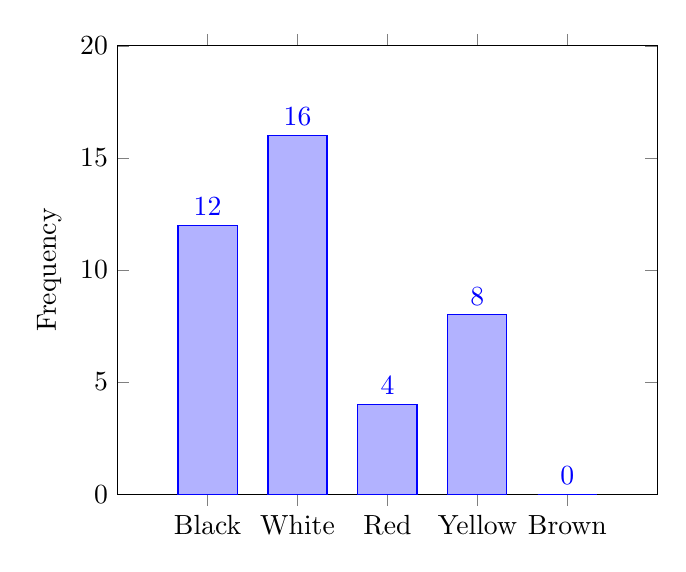
\begin{tikzpicture}
    \centering
    \begin{axis} [
      ylabel=Frequency,
      symbolic x coords={Black, White, Red, Yellow, Brown},
      ybar,
      xtick=data,
      ymin=0,
      enlarge y limits={value=0.25,upper},
      enlarge x limits=0.25,
      nodes near coords,
      bar width=0.75cm,
      ]
      \addplot coordinates {(Black, 12) (White, 16) (Red, 4) (Yellow, 8) (Brown, 0)};
    \end{axis}
  \end{tikzpicture}
  \caption{\label{plot:R8 colors bar plot} Colors of Audi R8s sold last year}
\end{figure}


%%%%%%%%%%%%%%%%%%%%%%%%%%%%%%%%%%%%%%%%%
\subsection{Relative frequencies}

In Figure \ref{plot:R8 colors bar plot}, we plotted the frequency counts. We can also use a bar plot to plot the \emph{relative} frequencies, as for example in Figure \ref{plot:R8 colors relative frequencies bar plot}

\begin{figure}[ht]
  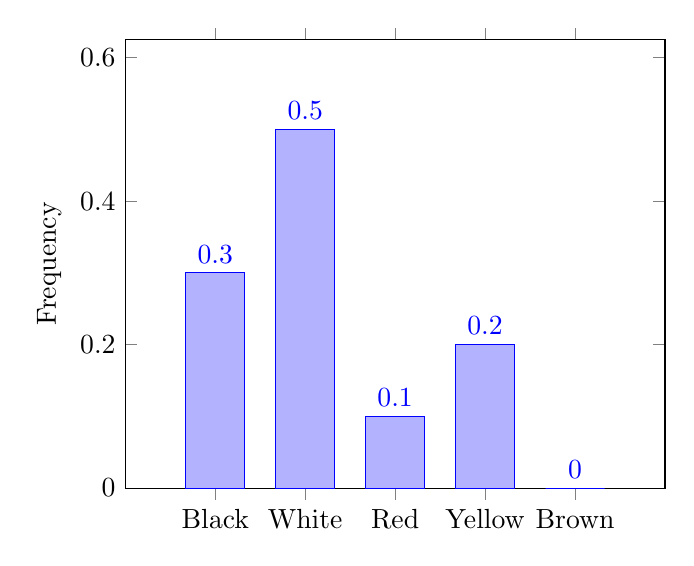
\begin{tikzpicture}
    \centering
    \begin{axis} [
      ylabel=Frequency,
      symbolic x coords={Black, White, Red, Yellow, Brown},
      ybar,
      xtick=data,
      ymin=0,
      enlarge y limits={value=0.25,upper},
      enlarge x limits=0.25,
      nodes near coords,
      bar width=0.75cm,
      ]
      \addplot coordinates {(Black, 0.3) (White, 0.5) (Red, 0.1) (Yellow, 0.2) (Brown, 0.0)};
    \end{axis}
  \end{tikzpicture}
  \caption{\label{plot:R8 colors relative frequencies bar plot} Colors of Audi R8s sold last year (relative frequencies)}
\end{figure}


%%%%%%%%%%%%%%%%%%%%%%%%%%%%%%%%%%%%%%%%%
\subsection{Order of bars}

The order of the bars does not matter in a bar plot. We can change them around. For example, compare Figure \ref{plot:R8 colors bar plot} and Figure \ref{plot:R8 colors bar plot 2}. Both of these are the same bar plot, since the order of the bars does not matter.

\begin{figure}[ht]
  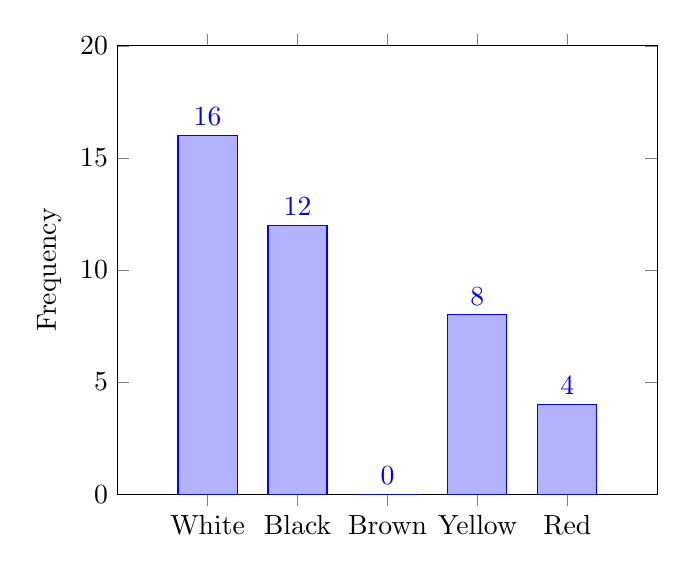
\begin{tikzpicture}
    \centering
    \begin{axis} [
      ylabel=Frequency,
      symbolic x coords={White, Black, Brown, Yellow, Red},
      ybar,
      xtick=data,
      ymin=0,
      enlarge y limits={value=0.25,upper},
      enlarge x limits=0.25,
      nodes near coords,
      bar width=0.75cm,
      ]
      \addplot coordinates {(White, 16) (Black, 12) (Brown, 0) (Yellow, 8) (Red, 4)};
    \end{axis}
  \end{tikzpicture}
  \caption{\label{plot:R8 colors bar plot 2} Colors of Audi R8s sold last year}
\end{figure}


%%%%%%%%%%%%%%%%%%%%%%%%%%%%%%%%%%%%%%%%%
\subsection{Sideways bar plots}

Bar plots can be drawn sideways too. That is, the bars can grow out sideways (horizontally) instead of upwards (vertically). Figure \ref{plot:R8 colors bar plot sideways} is the same as Figure \ref{plot:R8 colors bar plot}, but it is turned sideways.

\begin{figure}[ht]
  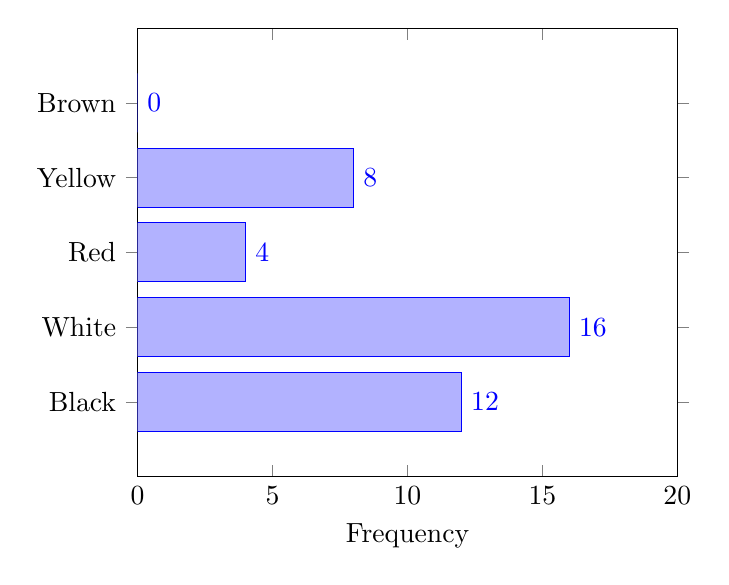
\begin{tikzpicture}
    \centering
    \begin{axis} [
      xlabel=Frequency,
      symbolic y coords={Black, White, Red, Yellow, Brown},
      xbar,
      ytick=data,
      xmin=0,
      enlarge x limits={value=0.25,upper},
      enlarge y limits=0.25,
      nodes near coords,
      bar width=0.75cm,
      ]
      \addplot coordinates {(12,Black) (16,White) (4,Red) (8,Yellow) (0,Brown)};
    \end{axis}
  \end{tikzpicture}
  \caption{\label{plot:R8 colors bar plot sideways} Colors of Audi R8s sold last year}
\end{figure}


%%%%%%%%%%%%%%%%%%%%%%%%%%%%%%%%%%%%%%%%%
\subsection{Summary}

Note some features about bar plots:

\begin{itemize}

  \item Bar plots visualize the \emph{frequencies} or \emph{relative frequencies} of a data set.

  \item The bars are \emph{spaced apart} a bit.
  
  \item The \emph{order} of the bars \emph{does not matter}. We could put the colors in any order, and it would still be the same bar plot.
  
  \item Since order does not matter, bar plots are best suited to plot values from a \emph{nominal scale}.
  
  \item Bar plots can be turned on their sides, so that the bars grow sideways (horizontally) rather than upwards (vertically).

\end{itemize}


%%%%%%%%%%%%%%%%%%%%%%%%%%%%%%%%%%%%%%%%%
%%%%%%%%%%%%%%%%%%%%%%%%%%%%%%%%%%%%%%%%%
\section{Line plots}

\vocab{Line plots} (also called line graphs or line charts) are much like bar plots, except instead of drawing bars, you just draw a dot where the top of each bar would be, and then you connect all the dots with a line. Here is the data from Table \ref{table:R8 colors} in a line plot:

\begin{figure}[ht]
  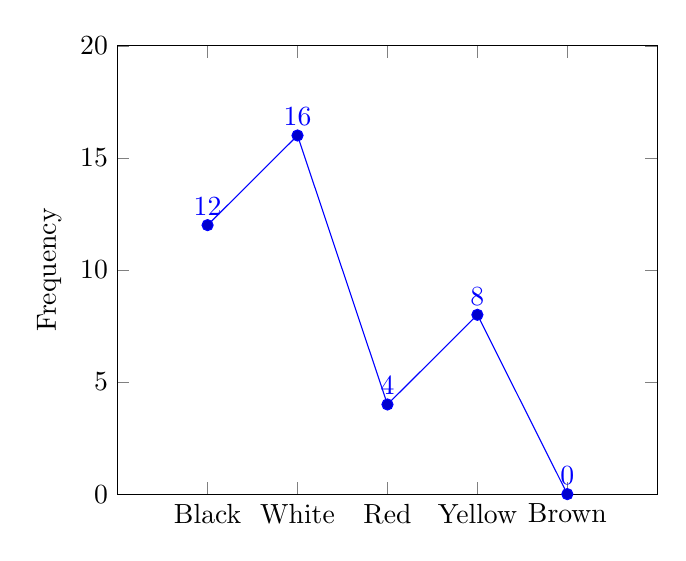
\begin{tikzpicture}
    \centering
    \begin{axis} [
      ylabel=Frequency,
      symbolic x coords={Black, White, Red, Yellow, Brown},
      xtick=data,
      ymin=0,
      enlarge y limits={value=0.25,upper},
      enlarge x limits=0.25,
      nodes near coords,
      ]
      \addplot coordinates {(Black, 12) (White, 16) (Red, 4) (Yellow, 8) (Brown, 0)};
    \end{axis}
  \end{tikzpicture}
  \caption{\label{plot:R8 colors line plot} Colors of Audi R8s sold last year}
\end{figure}


%%%%%%%%%%%%%%%%%%%%%%%%%%%%%%%%%%%%%%%%%
\subsection{The slope is meaningless}

Line plots have the same properties as bar plots. The line is there to show us the ``shape'' of the data. And indeed, if you imagine the area under the line filled, you can see how a line plot gives us a visual picture of the shape of the data. The peaks show us where the frequencies are clustered under.

That being said, do not read anything into the \emph{slope} of the line. The slope of a line going up or down suggests no ``trend'' in a line plot. Trending upwards or downwards is meaningless in a line plot, because a line plot is simply plotting the frequencies (or relative frequencies). 

Indeed, the colors in Figure \ref{plot:R8 colors line plot} fall on a \emph{nominal scale}, so there is no order between them. It is thus meaningless to think that there is any kind of growth from (say) ``Red'' to ``Yellow.'' Also, we can reorder the colors, and then the line plot looks entirely different! For example, look at Figure \ref{plot:R8 colors line plot 2}. It is the same data, but the colors are put in a different order, which makes the line look different. 

\begin{figure}[ht]
  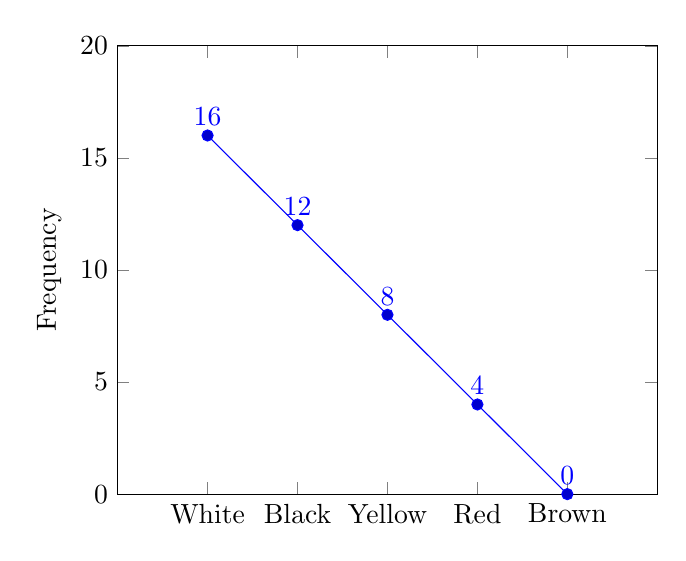
\begin{tikzpicture}
    \centering
    \begin{axis} [
      ylabel=Frequency,
      symbolic x coords={White, Black, Yellow, Red, Brown},
      xtick=data,
      ymin=0,
      enlarge y limits={value=0.25,upper},
      enlarge x limits=0.25,
      nodes near coords,
      ]
      \addplot coordinates {(White, 16) (Black, 12) (Yellow, 8) (Red, 4) (Brown, 0)};
    \end{axis}
  \end{tikzpicture}
  \caption{\label{plot:R8 colors line plot 2} Colors of Audi R8s sold last year}
\end{figure}

You may be thinking that the line in a line plot is too misleading, and so line plots are really quite useless. You may continue thinking this, if you like. A bar plot is always better.


%%%%%%%%%%%%%%%%%%%%%%%%%%%%%%%%%%%%%%%%%
%%%%%%%%%%%%%%%%%%%%%%%%%%%%%%%%%%%%%%%%%
\section{Histograms}

The most important kind of plot for visualizing frequencies is the \vocab{histogram}. A histogram looks similar to a bar plot, but the order of the bars is not arbitrary. In a historgram, the bars must be plotted in the order of the data values. Hence, to use a histogram, the data values must be ordered! In other words, histograms are used to plot data that falls on an \emph{ordinal scale} or higher. 

Consequently, a histogram cannot be used to visualize nominal scale data. If you make a histogram with nominal scale data, it's not really a histogram. It's just a bar plot.

Suppose we collect all the final exam scores for a Biology 101 class at a nearby university from last year. The frequency counts are displayed in Table \ref{table:Biology 101 scores}:

\begin{table}[ht]
  \begin{tabular}{| c | c || c | c || c | c |}
    \hline
    \textbf{Score} & \textbf{Frequency} & \textbf{Score} & \textbf{Frequency} & \textbf{Score} & \textbf{Frequency} \\ \hline
    0 & 4 & 67 & 6 & 85 & 8 \\ \hline
    23 & 1 & 69 & 1 & 86 & 2 \\ \hline
    25 & 2 & 70 & 4 & 87 & 4 \\ \hline
    49 & 1 & 72 & 1 & 89 & 12 \\ \hline
    54 & 2 & 73 & 2 & 90 & 10 \\ \hline
    58 & 1 & 76 & 4 & 91 & 9 \\ \hline
    60 & 1 & 77 & 8 & 92 & 7 \\ \hline
    63 & 1 & 78 & 5 & 96 & 2 \\ \hline
    64 & 2 & 80 & 4 & 97 & 5 \\ \hline
    65 & 2 & 83 & 6 & 98 & 2 \\ \hline
  \end{tabular}
  \caption{\label{table:Biology 101 scores}All Biology 101 final exam scores}  
\end{table}

There are a lot of values in this table. If we try to put this data into a bar plot, we would end up with something like Figure \ref{plot:Biology 101 scores bar plot}. There are just too many bars clustered on top of each other in that plot.

\begin{figure}[ht]
  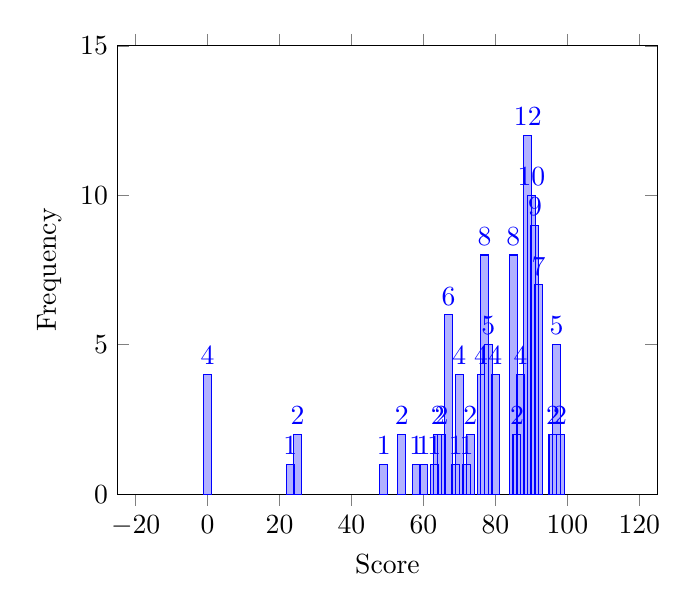
\begin{tikzpicture}
    \centering
    \begin{axis} [
      ylabel=Frequency,
      xlabel=Score,
      ybar,
      ymin=0,
      xmin=0,
      xmax=100,
      enlarge y limits={value=0.25,upper},
      enlarge x limits=0.25,
      nodes near coords,
      bar width=0.1cm,
      ]
      \addplot coordinates {
        (0, 4) (23, 1) (25, 2) (49, 1) (54, 2) (58, 1) (60, 1) (63, 1) (64, 2) (65, 2)
        (67, 6) (69, 1) (70, 4) (72, 1) (73, 2) (76, 4) (77, 8) (78, 5) (80, 4) (83 6)
        (85, 8) (86, 2) (87, 4) (89, 12) (90, 10) (91, 9) (92, 7) (96, 2) (97, 5) (98, 2)
      };
    \end{axis}
  \end{tikzpicture}
  \caption{\label{plot:Biology 101 scores bar plot} Colors of Audi R8s sold last year}
\end{figure}

Perhaps we break the total 100 points up by 20s, and then we could clump all scores from 0 to 19 together into one count, and do the same for scores from 20--39, 40--59, 60--79, and 80--99.

How many scores fall between 0 and 19? There are four (all zeros). How many fall between 20 and 39? There are three (one score of 23, and two scores of 25). We can do the same for the other chunks, to get a frequency count like we see in Table \ref{table:Biology 101 scores by 20s}.

\begin{table}[ht]
  \begin{tabular}{| c | c |}
    \hline
    \textbf{Score} & \textbf{Frequency} \\ \hline
    0--19 & 4 \\ \hline
    20--39 & 3 \\ \hline
    40--59 & 4 \\ \hline
    60--79 & 37 \\ \hline
    80--99 & 72 \\ \hline
  \end{tabular}
  \caption{\label{table:Biology 101 scores by 20s}Biology 101 final exam scores, grouped by 20s}  
\end{table}

If we make a bar chart of this, we end up with something that looks like Figure \ref{plot:Biology 101 scores by 20s bar plot}.

\begin{figure}[ht]
  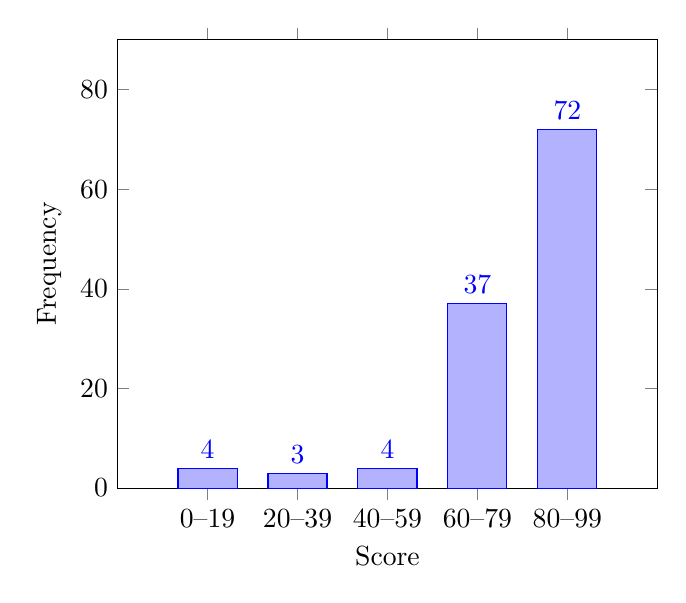
\begin{tikzpicture}
    \centering
    \begin{axis} [
      ylabel=Frequency,
      xlabel=Score,
      ybar,
      ymin=0,
      xtick=data,
      symbolic x coords={0--19, 20--39, 40--59, 60--79, 80--99},
      enlarge y limits={value=0.25,upper},
      enlarge x limits=0.25,
      nodes near coords,
      bar width=0.75cm,
      ]
      \addplot coordinates {
        (0--19, 4) (20--39, 3) (40--59, 4) (60--79, 37) (80--99, 72)
      };
    \end{axis}
  \end{tikzpicture}
  \caption{\label{plot:Biology 101 scores by 20s bar plot} Biology 101 scores}
\end{figure}

If we slide the bars right next to each other, we turn the plot into a \vocab{histogram}. This is done in Figure \ref{plot:Biology 101 scores by 20s histogram}.

\begin{figure}[ht]
  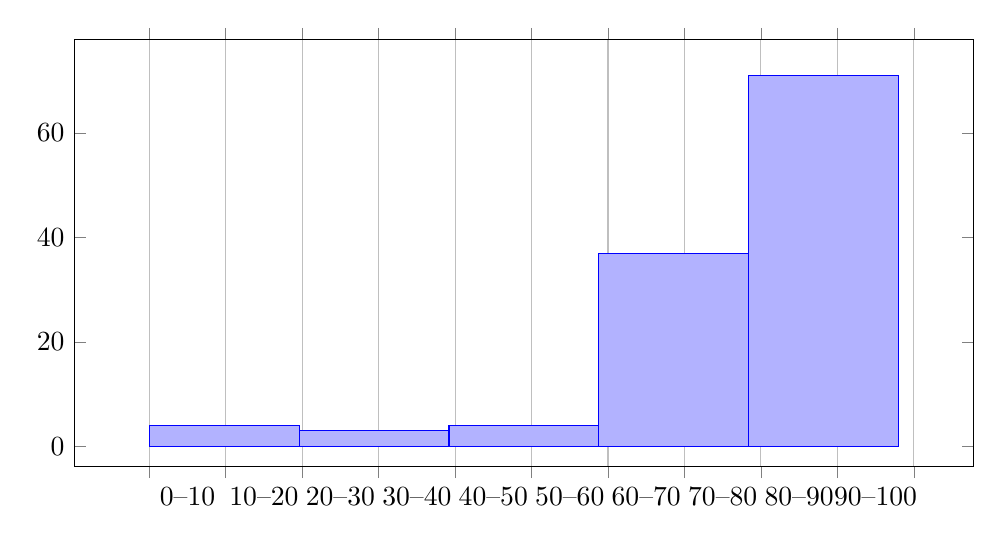
\begin{tikzpicture}
    \centering
    \begin{axis} [
      height=7cm,
      width=13cm,
      ybar interval,
      xtick=,
      xticklabel=\pgfmathprintnumber\tick--\pgfmathprintnumber\nexttick,
      ]
      \addplot+ [hist={bins=5}]
        table [row sep=\\, y index=0] {
          data \\
           0 \\ 0 \\ 0 \\ 0 \\ 23 \\ 25 \\ 25 \\ 49 \\ 54 \\ 54 \\
 58 \\ 60 \\ 63 \\ 64 \\ 64 \\ 65 \\ 65 \\ 
 67 \\ 67 \\ 67 \\ 67 \\ 67 \\ 67 \\ 69 \\
 70 \\ 70 \\ 70 \\ 70 \\ 72 \\ 73 \\ 73 \\
 76 \\ 76 \\ 76 \\ 76 \\ 77 \\ 77 \\ 77 \\ 77 \\ 77 \\ 77 \\ 77 \\ 77 \\
 78 \\ 78 \\ 78 \\ 78 \\ 78 \\ 80 \\ 80 \\ 80 \\ 80 \\
 83 \\ 83 \\ 83 \\ 83 \\ 83 \\ 83 \\ 
 85 \\ 85 \\ 85 \\ 85 \\ 85 \\ 85 \\ 85 \\ 85 \\ 86 \\ 86 \\
 87 \\ 87 \\ 87 \\ 87 \\ 
 89 \\ 89 \\ 89 \\ 89 \\ 89 \\ 89 \\ 89 \\ 89 \\ 89 \\ 89 \\ 89 \\ 89 \\
 90 \\ 90 \\ 90 \\ 90 \\ 90 \\ 90 \\ 90 \\ 90 \\ 90 \\ 90 \\
 91 \\ 91 \\ 91 \\ 91 \\ 91 \\ 91 \\ 91 \\ 91 \\ 91 \\
 92 \\ 92 \\ 92 \\ 92 \\92 \\ 92 \\ 92 \\ 96 \\ 96 \\
 97 \\ 97 \\ 97 \\ 97 \\ 97 \\ 98 \\ 98 \\
      };
    \end{axis}
  \end{tikzpicture}
  \caption{\label{plot:Biology 101 scores by 20s histogram} Biology 101 scores (interval 20)}
\end{figure}

So a histogram is just like a bar plot, but the values are grouped into intervals (in our example, the interval is 20), and the bars are drawn touching each other.

A histogram lets us see the shape or distribution of the data, in the sense that it tells us where most of the values occur. In Figure \ref{plot:Biology 101 scores by 20s histogram}, we can see immediately that most of the scores occur in the 80s and 90s, and then another, smaller group of scores occur in the 60s and 70s, while very few scores were lower than that.


%%%%%%%%%%%%%%%%%%%%%%%%%%%%%%%%%%%%%%%%%
\subsection{Changing the interval}

In Figure \ref{plot:Biology 101 scores by 20s histogram}, the interval is pretty wide. We can make the interval smaller, and that may give us a slightly clearer picture. In Figure \ref{plot:Biology 101 scores by 10s histogram}, the interval is 10 (instead of 20 as it was before). 

\begin{figure}[ht]
  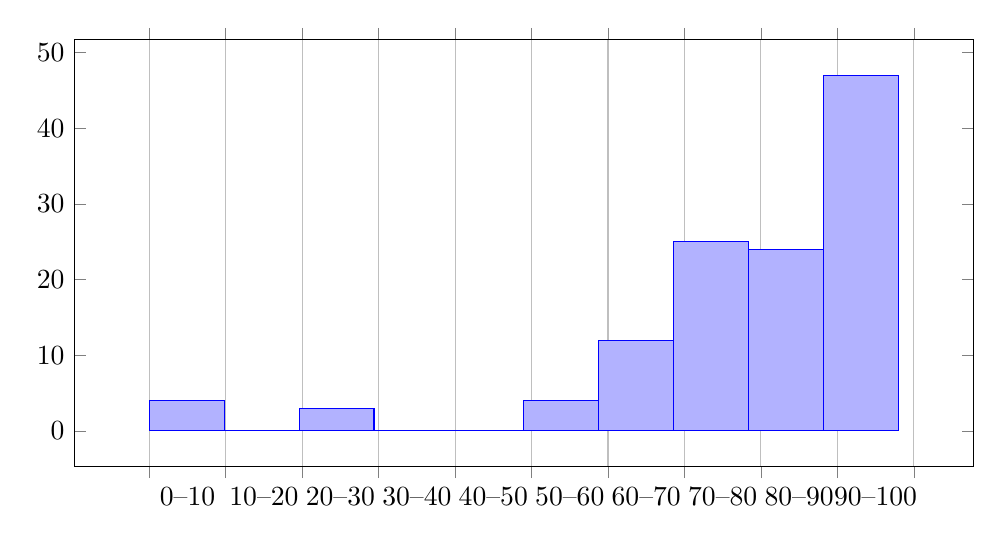
\begin{tikzpicture}
    \centering
    \begin{axis} [
      height=7cm,
      width=13cm,
      ybar interval,
      xtick=,
      xticklabel=\pgfmathprintnumber\tick--\pgfmathprintnumber\nexttick,
      ]
      \addplot+ [hist={bins=10}]
        table [row sep=\\, y index=0] {
          data \\
           0 \\ 0 \\ 0 \\ 0 \\ 23 \\ 25 \\ 25 \\ 49 \\ 54 \\ 54 \\
 58 \\ 60 \\ 63 \\ 64 \\ 64 \\ 65 \\ 65 \\ 
 67 \\ 67 \\ 67 \\ 67 \\ 67 \\ 67 \\ 69 \\
 70 \\ 70 \\ 70 \\ 70 \\ 72 \\ 73 \\ 73 \\
 76 \\ 76 \\ 76 \\ 76 \\ 77 \\ 77 \\ 77 \\ 77 \\ 77 \\ 77 \\ 77 \\ 77 \\
 78 \\ 78 \\ 78 \\ 78 \\ 78 \\ 80 \\ 80 \\ 80 \\ 80 \\
 83 \\ 83 \\ 83 \\ 83 \\ 83 \\ 83 \\ 
 85 \\ 85 \\ 85 \\ 85 \\ 85 \\ 85 \\ 85 \\ 85 \\ 86 \\ 86 \\
 87 \\ 87 \\ 87 \\ 87 \\ 
 89 \\ 89 \\ 89 \\ 89 \\ 89 \\ 89 \\ 89 \\ 89 \\ 89 \\ 89 \\ 89 \\ 89 \\
 90 \\ 90 \\ 90 \\ 90 \\ 90 \\ 90 \\ 90 \\ 90 \\ 90 \\ 90 \\
 91 \\ 91 \\ 91 \\ 91 \\ 91 \\ 91 \\ 91 \\ 91 \\ 91 \\
 92 \\ 92 \\ 92 \\ 92 \\92 \\ 92 \\ 92 \\ 96 \\ 96 \\
 97 \\ 97 \\ 97 \\ 97 \\ 97 \\ 98 \\ 98 \\
      };
    \end{axis}
  \end{tikzpicture}
  \caption{\label{plot:Biology 101 scores by 10s histogram} Biology 101 scores (interval 10)}
\end{figure}

With the interval set to 10, we can see the distribution of the data even better. For example, look at the scores from 0 to 20. Before, we could see that there were 4 scores in that interval. But now, we can see that all of the scores occur in the interval from 0 to 10, and no scores occur in the interval from 10 to 20. Similarly, look at the scores that occur between 80 and 100. Before, we could see only that there were a lot of scores in the 80s and 90s. Now we can see that most of them are in the 90s.

We can make the interval even smaller if we want. For example, we could set it to 5, like in Figure \ref{plot:Biology 101 scores by 5s histogram}

\begin{figure}[ht]
  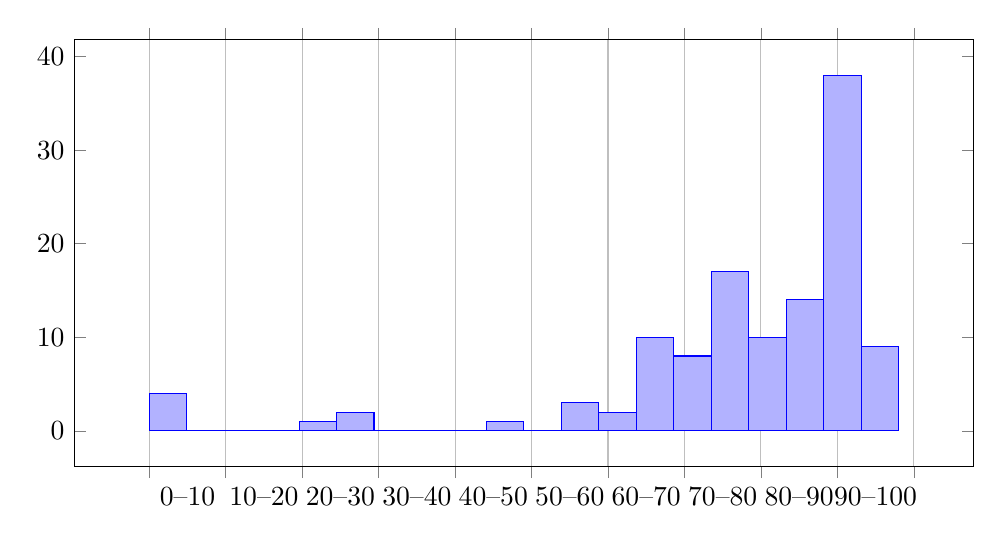
\begin{tikzpicture}
    \centering
    \begin{axis} [
      height=7cm,
      width=13cm,
      ybar interval,
      xtick=,
      xticklabel=\pgfmathprintnumber\tick--\pgfmathprintnumber\nexttick,
      ]
      \addplot+ [hist={bins=20}]
        table [row sep=\\, y index=0] {
          data \\
           0 \\ 0 \\ 0 \\ 0 \\ 23 \\ 25 \\ 25 \\ 49 \\ 54 \\ 54 \\
 58 \\ 60 \\ 63 \\ 64 \\ 64 \\ 65 \\ 65 \\ 
 67 \\ 67 \\ 67 \\ 67 \\ 67 \\ 67 \\ 69 \\
 70 \\ 70 \\ 70 \\ 70 \\ 72 \\ 73 \\ 73 \\
 76 \\ 76 \\ 76 \\ 76 \\ 77 \\ 77 \\ 77 \\ 77 \\ 77 \\ 77 \\ 77 \\ 77 \\
 78 \\ 78 \\ 78 \\ 78 \\ 78 \\ 80 \\ 80 \\ 80 \\ 80 \\
 83 \\ 83 \\ 83 \\ 83 \\ 83 \\ 83 \\ 
 85 \\ 85 \\ 85 \\ 85 \\ 85 \\ 85 \\ 85 \\ 85 \\ 86 \\ 86 \\
 87 \\ 87 \\ 87 \\ 87 \\ 
 89 \\ 89 \\ 89 \\ 89 \\ 89 \\ 89 \\ 89 \\ 89 \\ 89 \\ 89 \\ 89 \\ 89 \\
 90 \\ 90 \\ 90 \\ 90 \\ 90 \\ 90 \\ 90 \\ 90 \\ 90 \\ 90 \\
 91 \\ 91 \\ 91 \\ 91 \\ 91 \\ 91 \\ 91 \\ 91 \\ 91 \\
 92 \\ 92 \\ 92 \\ 92 \\92 \\ 92 \\ 92 \\ 96 \\ 96 \\
 97 \\ 97 \\ 97 \\ 97 \\ 97 \\ 98 \\ 98 \\
      };
    \end{axis}
  \end{tikzpicture}
  \caption{\label{plot:Biology 101 scores by 5s histogram} Biology 101 scores (interval 5)}
\end{figure}

We can keep making the interval smaller and smaller, but there is a point where there are too many intervals and the bars are too numerous to really tell us much (just like the initial bar plot we did for the scores). A histogram is useful because it \emph{summarize} the data for us quickly. By grouping the values into intervals, we summarize the data. When we make the intervals too small, we summarize less and less. So use good judgment when constructing a histogram. Try to find the interval that shows the right balance of information.The interval should be not too small, but not too big either.


%%%%%%%%%%%%%%%%%%%%%%%%%%%%%%%%%%%%%%%%%
\subsection{Summary}

Here are the points to remember about a histogram:

\begin{itemize}
  
  \item Histograms can be used to visualize \emph{frequencies} or \emph{relative frequencies}.
  
  \item Histograms should be used to visualize data that falls on an \emph{ordinal scale} or higher. 
  
  \item Nominal scale data \emph{cannot} be plotted with a histogram. 
  
  \item Histograms group the values into \emph{intervals}, which can be adjusted to suit your needs.
  
  \item The bars \emph{touch} (there is no space between them).

\end{itemize}


%%%%%%%%%%%%%%%%%%%%%%%%%%%%%%%%%%%%%%%%%
%%%%%%%%%%%%%%%%%%%%%%%%%%%%%%%%%%%%%%%%%
\section{Frequency polygons}

A \vocab{frequency polygon} is just like a histogram, except instead of bars, you put a dot at the top of where the bar would be, and you connect the dots with a line. If we convert the bars from Figure \ref{plot:Biology 101 scores by 20s histogram} into dots and connect the lines, we get the plot in Figure \ref{plot:Biology 101 scores by 20s polygon beta}.

\begin{figure}[ht]
  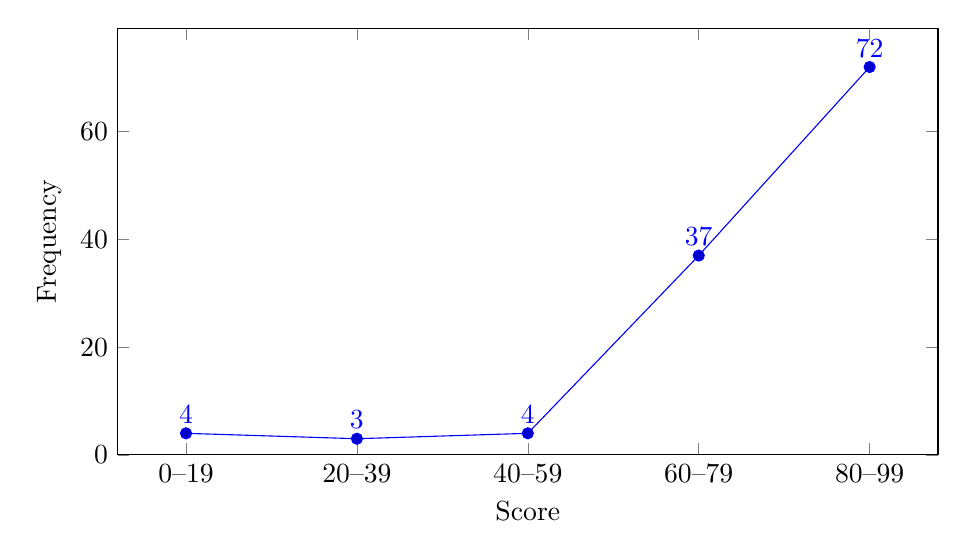
\begin{tikzpicture}
    \centering
    \begin{axis} [
      height=7cm,
      width=12cm,
      ylabel=Frequency,
      xlabel=Score,
      ymin=0,
      xtick=data,
      symbolic x coords={0--19, 20--39, 40--59, 60--79, 80--99},
      enlarge y limits={value=0.1,upper},
      nodes near coords,
      ]
      \addplot+ [sharp plot] coordinates {
        (0--19, 4) (20--39, 3) (40--59, 4) (60--79, 37) (80--99, 72)
      };
    \end{axis}
  \end{tikzpicture}
  \caption{\label{plot:Biology 101 scores by 20s polygon beta} Biology 101 scores}
\end{figure}

The only thing about Figure \ref{plot:Biology 101 scores by 20s polygon beta} is that it does not form a polygon, because the ends of the line don't connect to the x-axis. To fix this, we just connect each end of the line to the bottom/x-axis at some point before/after the values we are plotting. Then we have a complete frequency polygon, as in Figure \ref{plot:Biology 101 scores by 20s polygon}.

\begin{figure}[ht]
  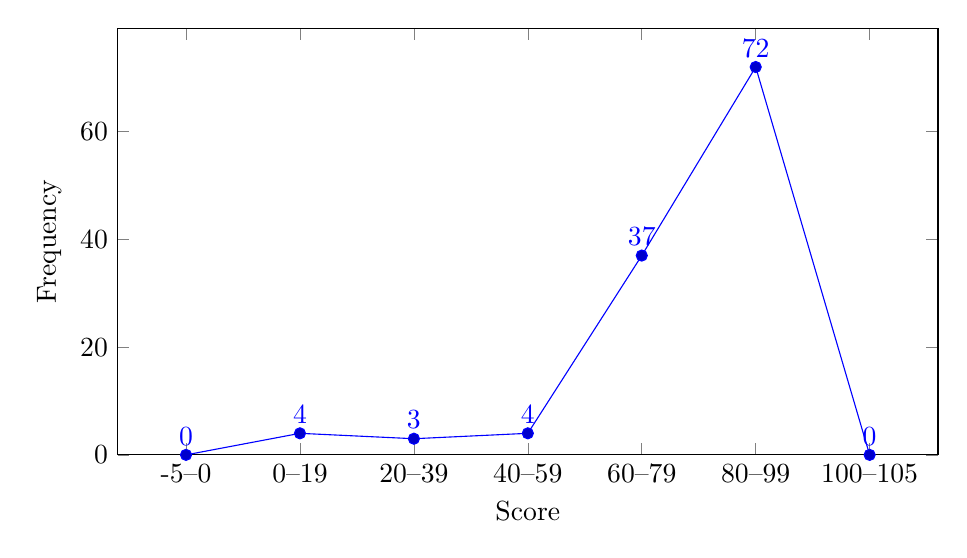
\begin{tikzpicture}
    \centering
    \begin{axis} [
      height=7cm,
      width=12cm,
      ylabel=Frequency,
      xlabel=Score,
      ymin=0,
      xtick=data,
      symbolic x coords={-5--0, 0--19, 20--39, 40--59, 60--79, 80--99, 100--105},
      enlarge y limits={value=0.1,upper},
      nodes near coords,
      ]
      \addplot+ [sharp plot] coordinates {
        (-5--0, 0) (0--19, 4) (20--39, 3) (40--59, 4) (60--79, 37) (80--99, 72) (100--105, 0)
      };
    \end{axis}
  \end{tikzpicture}
  \caption{\label{plot:Biology 101 scores by 20s polygon} Biology 101 scores}
\end{figure}

Much like the histogram with an interval of 20, Figure \ref{plot:Biology 101 scores by 20s polygon} doesn't give us much information. We can make the intervals smaller, to get a clearer picture. If we convert Figure \ref{plot:Biology 101 scores by 10s histogram} into a frequency polygon, we get the plot in Figure \ref{plot:Biology 101 scores by 10s polygon}.

\begin{figure}[ht]
  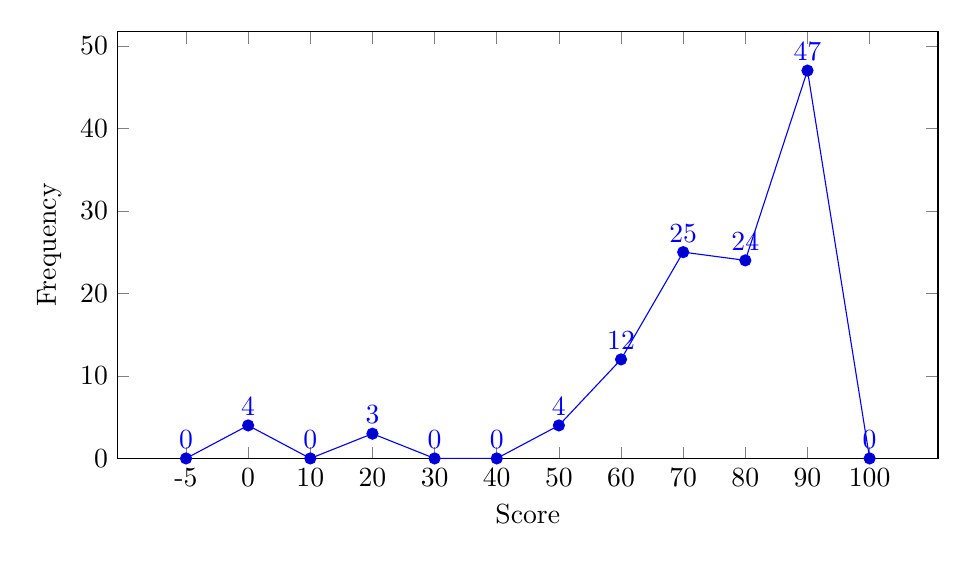
\begin{tikzpicture}
    \centering
    \begin{axis} [
      height=7cm,
      width=12cm,
      ylabel=Frequency,
      xlabel=Score,
      ymin=0,
      xtick=data,
      symbolic x coords={-5, 0, 10, 20, 30, 40, 50, 60, 70, 80, 90, 100},
      enlarge y limits={value=0.1,upper},
      nodes near coords,
      ]
      \addplot+ [sharp plot] coordinates {
        (-5, 0) (0, 4) (10, 0) (20, 3) (30, 0) (40, 0) (50, 4) (60, 12) (70, 25) (80, 24) (90, 47) (100, 0)
      };
    \end{axis}
  \end{tikzpicture}
  \caption{\label{plot:Biology 101 scores by 10s polygon} Biology 101 scores}
\end{figure}

And if we convert Figure \ref{plot:Biology 101 scores by 5s histogram} into a frequency polygon, we get the plot in Figure \ref{plot:Biology 101 scores by 5s polygon}.

\begin{figure}[ht]
  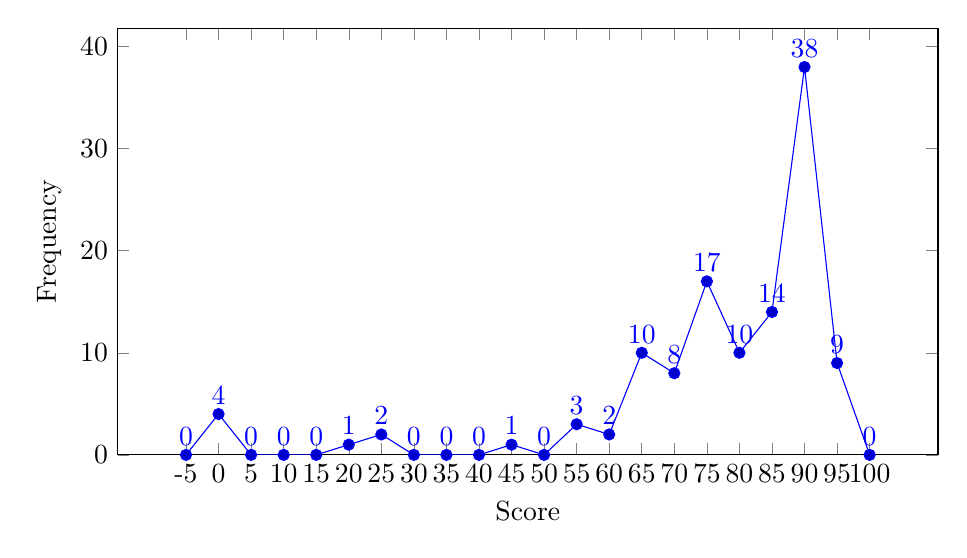
\begin{tikzpicture}
    \centering
    \begin{axis} [
      height=7cm,
      width=12cm,
      ylabel=Frequency,
      xlabel=Score,
      ymin=0,
      xtick=data,
      symbolic x coords={-5, 0, 5, 10, 15, 20, 25, 30, 35, 40, 45, 50, 55, 60, 65, 70, 75, 80, 85, 90, 95, 100},
      enlarge y limits={value=0.1,upper},
      nodes near coords,
      ]
      \addplot+ [sharp plot] coordinates {
        (-5, 0) (0, 4) (5, 0) (10, 0) (15, 0) (20, 1) (25, 2) (30, 0) (35, 0) (40, 0)
        (45, 1) (50, 0) (55, 3) (60, 2) (65, 10) (70, 8) (75, 17) (80, 10) (85, 14)
        (90, 38) (95, 9) (100, 0)
      };
    \end{axis}
  \end{tikzpicture}
  \caption{\label{plot:Biology 101 scores by 5s polygon} Biology 101 scores}
\end{figure}

Frequency polygons basically show the same information as histogram. One should always use a histogram when possible. But there is one kind of case where frequency polygons are more useful than histograms, and that is when you want to plot two or more data sets at the same time. Frequency polygons are useful here because you can lay down one (or more) on top of another, and this lets us see two (or more) frequency distributions compared against each other.

For example, suppose we take all the scores from the previous year's Biology 101 class, and plot that polygon on top of this years. Then we might have a plot like in Figure \ref{plot:Biology 101 scores by 10s two polygons}.

\begin{figure}[ht]
  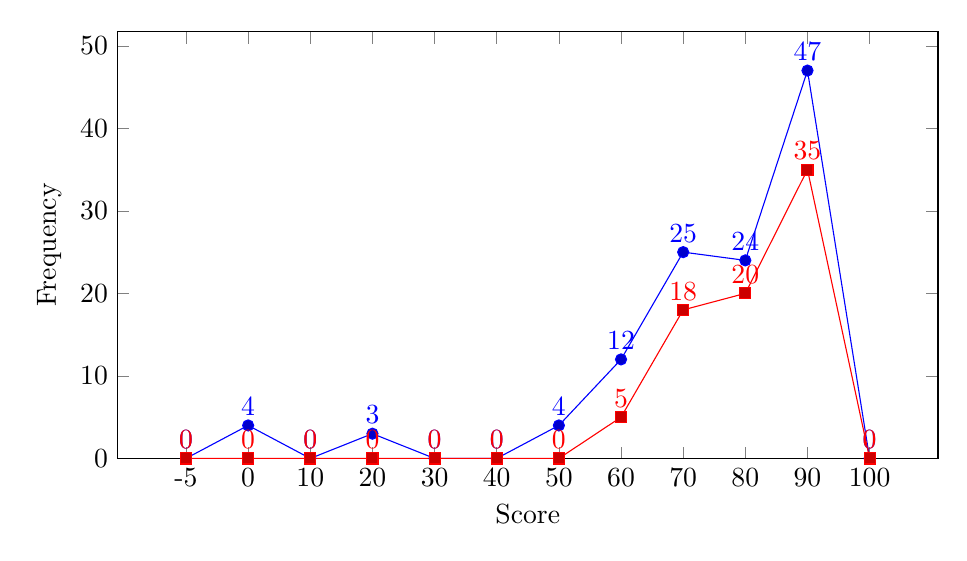
\begin{tikzpicture}
    \centering
    \begin{axis} [
      height=7cm,
      width=12cm,
      ylabel=Frequency,
      xlabel=Score,
      ymin=0,
      xtick=data,
      symbolic x coords={-5, 0, 10, 20, 30, 40, 50, 60, 70, 80, 90, 100},
      enlarge y limits={value=0.1,upper},
      nodes near coords,
      ]
      \addplot+ [sharp plot] coordinates {
        (-5, 0) (0, 4) (10, 0) (20, 3) (30, 0) (40, 0) (50, 4) (60, 12) (70, 25) (80, 24) (90, 47) (100, 0)
      };
      \addplot+ [sharp plot] coordinates {
        (-5, 0) (0, 0) (10, 0) (20, 0) (30, 0) (40, 0) (50, 0) (60, 5) (70, 18) (80, 20) (90, 35) (100, 0)
      };
    \end{axis}
  \end{tikzpicture}
  \caption{\label{plot:Biology 101 scores by 10s two polygons} Biology 101 scores last year and this year (interval 10)}
\end{figure}


%%%%%%%%%%%%%%%%%%%%%%%%%%%%%%%%%%%%%%%%%
\subsection{Summary}

Here are the points to remember about frequency polygons:

\begin{itemize}

  \item A frequency polygon is much like a histogram.
  
  \item A histogram should always be used instead of a frequency polygon, except when you want to plot two or more data sets at the same time. Then a frequency polygon should be used.

\end{itemize}


%%%%%%%%%%%%%%%%%%%%%%%%%%%%%%%%%%%%%%%%%
%%%%%%%%%%%%%%%%%%%%%%%%%%%%%%%%%%%%%%%%%
\section{Time series plots}

A \vocab{time series plot} (also called a \emph{time series graph}) plots frequencies over time. Suppose we want to plot the number of days that employees took off for each month from last year. We can put the months on the x-axis, and the days taken off on the y-axis, and draw a line through all the points. Figure \ref{plot:Employee days off time series plot} is an example of what this might look like.

\begin{figure}[ht]
  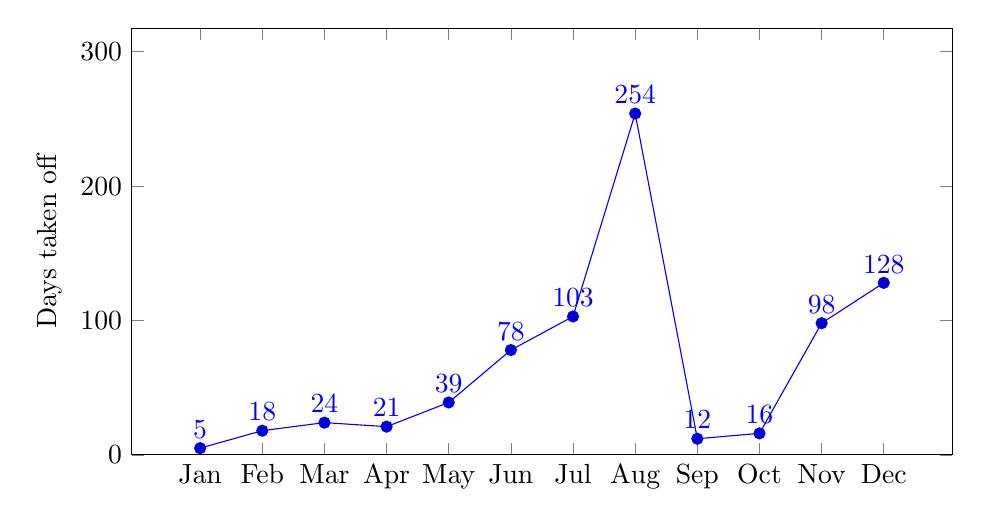
\begin{tikzpicture}
    \centering
    \begin{axis} [
      height=7cm,
      width=12cm,
      ylabel=Days taken off,
      ymin=0,
      xtick=data,
      symbolic x coords={Jan, Feb, Mar, Apr, May, Jun, Jul, Aug, Sep, Oct, Nov, Dec},
      enlarge y limits={value=0.25,upper},
      nodes near coords,
      ]
      \addplot+ [sharp plot] coordinates {
        (Jan, 5) (Feb, 18) (Mar, 24) (Apr, 21) (May, 39) (Jun, 78) (Jul, 103) (Aug, 254) (Sep, 12) (Oct, 16) (Nov, 98) (Dec, 128)
      };
    \end{axis}
  \end{tikzpicture}
  \caption{\label{plot:Employee days off time series plot} Employee days taken off (last year)}
\end{figure}


%%%%%%%%%%%%%%%%%%%%%%%%%%%%%%%%%%%%%%%%%
\subsection{Summary}

Here are the points to remember about time series plots:

\begin{itemize}

  \item A time series plot should be used when you want to visualize \emph{frequencies} or \emph{relative frequencies} over time.

\end{itemize}



\end{document}
